% !TEX root = handbook-physics.tex
% !TEX TS-program = pdflatex
% !TEX encoding = UTF-8 Unicode






\chapter{Magnetic Materials In A Magnetic Field}
\label{ch-26}
\zhtitle{磁场中的磁性材料}

\section{Magnetic Moments of Electrons and Atoms}
\label{sec-26.1}
\zhtitle{电子和原子的磁矩}


\subsection{}\label{26.1.1} \redem{Magnetic materials} are all substances capable of acquiring magnetic properties, i.e. of being magnetized, in an external magnetic field. This means that they can set up their own magnetic field. The magnetic properties of substances are determined by the magnetic properties of their electrons and atoms.\sidenote{The magnetic properties of atomic nuclei are dealt with in \ssect{42.1.6}.} Magnetic materials are divided according to their magnetic properties into three main groups: diamagnetic \ssect{26.3.2}, para­ magnetic \ssect{26.3.5} and ferromagnetic \ssect{26.5.1} materials. 
\zhpar{\redem{磁性材料}是指所有能够在外磁场中获得磁性，即能够被磁化的物质。这意味着它们能够建立自身的磁场。物质的磁性质由其电子和原子的磁性质决定。按磁性质，磁性材料可分为三大类：抗磁性物质 \ssect{26.3.2}、顺磁性物质 \ssect{26.3.5} 和铁磁性物质 \ssect{26.5.1}。}
\zhpar{注：原子核的磁性质见 \ssect{42.1.6}。}

\subsection{}\label{26.1.2} The motion of an electron along its orbit in an atom is equivalent to a certain closed loop carrying a current (\redem{orbital current}). According to \ssect{23.3.4}, the \redem{orbital magnetic moment} $\vb{p}_{m}$ of an electron equals 
\zhpar{原子中电子沿其轨道的运动，等效于一个闭合的电流回路（\redem{轨道电流}）。根据 \ssect{23.3.4}，电子的\redem{轨道磁矩} $\vb{p}_{m}$ 等于：}
\begin{align*}%
\vb{p}_{m} & = IS \vu{n} && \text{(in SI units),} \\
\vb{p}_{m} & =  \frac{1}{c} IS \vu{n} && \text{(in Gaussian units)},
\end{align*}
where $I = e\nu$ is the current, $e$ is the magnitude of the charge of the electron, $nu$ is the number of revolutions of the electron along its orbit in unit time, $S$ is the area of the electron orbit, $\vu{n}$ is a unit vector of the normal to area $S$, and $c$ is the electrodynamic constant \ssect{23.2.2}.
\zhpar{式中 $I = e\nu$ 为电流，$e$ 为电子电荷的绝对值，$nu$ 为电子在单位时间内沿轨道运行的圈数，$S$ 为电子轨道的面积，$\vu{n}$ 为面积 $S$ 法线方向的单位矢量，$c$ 为电动力学常量 \ssect{23.2.2}。}

\begin{marginfigure}%[-2cm]
\centering
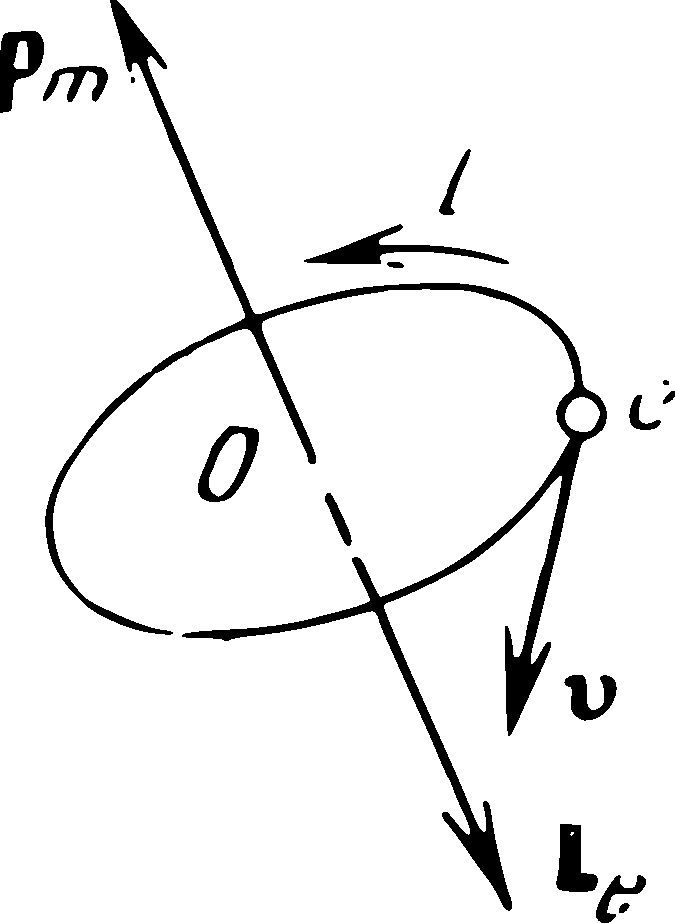
\includegraphics[width=0.6\textwidth]{figs/ch-26/fig-26-01.pdf}
\sidecaption{Orientation of vectors $\vb{p}_{m}$ and $\vb{L}_{e}$.\zhcap{矢量 $\vb{p}_{m}$ 与 $\vb{L}_{e}$ 的方向。}\label{fig-26-01}}
\end{marginfigure}

An electron moving along its orbit has an orbital angular momentum $\vb{L}_{e}$ \ssect{4.1.4}. The orbital magnetic moment is proportion­al to the orbital angular momentum:
\zhpar{沿轨道运动的电子具有轨道角动量 $\vb{L}_{e}$ \ssect{4.1.4}。轨道磁矩与轨道角动量成正比：}
\begin{equation*}%
\vb{p}_{m} = \gamma \vb{L}_{e},
\end{equation*}
where
\zhpar{式中：}
\begin{align*}%
\gamma & = - \frac{e}{2m} && \text{(in SI units),} \\
\gamma & =  - \frac{e}{2mc} && \text{(in Gaussian units)},
\end{align*}
The quantity $\gamma$ is called the \redem{gyromagnetic ratio of orbital mo­ments}.
\zhpar{量 $\gamma$ 称为\redem{轨道磁矩的旋磁比}。}

In the last formulas $m$ is the mass of the electron, $e$ is the magnitude of its charge, and $c$ is the electrodynamic constant \ssect{23.2.2}.
\zhpar{上述公式中，$m$ 为电子的质量，$e$ 为其电荷的绝对值，$c$ 为电动力学常量 \ssect{23.2.2}。}




Vectors $\vb{p}_{m}$ and $\vb{L}_{e}$ are opposite in direction and are perpendicular to the orbital plane of the electron (\figr{fig-26-01}). 
\zhpar{矢量 $\vb{p}_{m}$ 与 $\vb{L}_{e}$ 方向相反，且均垂直于电子的轨道平面（见\figr{fig-26-01}）。}

\subsection{}\label{26.1.3} An electron has an \redem{intrinsic angular momentum} $s$, which is called the spin of the electron. The magnitude of the electron spin is
\zhpar{电子具有\redem{固有角动量} $s$，称为电子的自旋。电子自旋的大小为：}
\begin{equation*}%
s = \frac{\sqrt{3}}{2} \, \frac{h}{2\pi} = \frac{\sqrt{3}}{2}  \hbar,
\end{equation*}
where $\hbar$ is Planck's constant (Appendix~II), and $\hbar = h/2\pi$. The most important feature of electron spin is that it has only two projections on the direction of vector $\vb{B}$ of magnetic induction.\sidenote{Regardless of whether it is an external magnetic field set up, for instance, by current-carrying conductors, or the internal magnetic field of the substance itself \ssect{26.4.2}.} Thus
\zhpar{式中 $\hbar$ 为普朗克常量（附录 II），且 $\hbar = h/2\pi$。电子自旋最重要的特征是，它在磁感应强度矢量 $\vb{B}$ 的方向上只有两个投影值。于是有：}
\zhpar{注：无论磁场是由载流导体等建立的外磁场，还是物质本身的内禀磁场 \ssect{26.4.2}。}
\begin{equation*}%
s_{B} = \pm \frac{\hbar}{2}.
\end{equation*}

\subsection{}\label{26.1.4} Electron spin $s$ corresponds to the spin magnetic moment $\vb{p}_{ms}$ which is proportional to the spin and opposite in direction. Thus
\zhpar{电子自旋 $s$ 对应于自旋磁矩 $\vb{p}_{ms}$，它与自旋成正比且方向相反。于是有：}
\begin{equation*}%
\vb{p}_{ms} = \gamma_{s}\,s.
\end{equation*}
The quantity $\gamma_{s}$ is called the \redem{gyromagnetic ratio of spin moments}:
\zhpar{量 $\gamma_{s}$ 称为\redem{自旋磁矩的旋磁比}：}
\begin{align*}%
\gamma & = - \frac{e}{m} && \text{(in SI units),} \\
\gamma & =  - \frac{e}{mc} && \text{(in Gaussian units)},
\end{align*}
where the notation is the same as in \ssect{26.1.2}.
\zhpar{式中符号的含义与 \ssect{26.1.2} 中相同。}


The projection of the electron spin magnetic moment on the direction of the field \ssect{26.1.3} equals
\zhpar{电子自旋磁矩在磁场方向（\ssect{26.1.3}）上的投影等于：}
\begin{align*}%
p_{msB} & = \pm \frac{e \hbar}{2m} && \text{(in SI units),} \\
p_{msB} & =  \pm \frac{e \hbar}{2mc} && \text{(in Gaussian units)},
\end{align*}
where $\mu_{B}$ is called the \redem{Bohr magneton}, and is a unit for measuring magnetic moments (Appendix~II).
\zhpar{式中 $\mu_{B}$ 称为\redem{玻尔磁子}，是度量磁矩的单位（附录 II）。}

\subsection{}\label{26.1.5} The information presented in \ssect{26.1.1} through \ssect{26.1.4} is valid for each of the $Z$ electrons in an atom. The number $Z$ coincides with the atomic number in Mendeleev's periodic table \ssect{39.3.5}.
\zhpar{\ssect{26.1.1} 至 \ssect{26.1.4} 中的内容对原子中的每一个电子（共 $Z$ 个）都成立。数 $Z$ 与门捷列夫周期表中的原子序数相同 \ssect{39.3.5}。}

The \redem{orbital magnetic moment} $\vb{P}_{m}$ of an atom is the vector sum of the orbital magnetic moments $\vb{p}_{m}$ of all its electrons. Thus
\zhpar{原子的\redem{轨道磁矩} $\vb{P}_{m}$ 等于其全部电子的轨道磁矩 $\vb{p}_{m}$ 的矢量和。于是有：}
\begin{equation*}%
\vb{P}_{m} = \sum_{i = 1}^{Z} \vb{p}_{mi}.
\end{equation*}
The \emph{orbital angular momentum} $L$ of the atom is the vector sum of the orbital angular momenta $\vb{L}_{e}$ of all $Z$ electrons. Thus
\zhpar{原子的\emph{轨道角动量} $L$ 等于全部 $Z$ 个电子的轨道角动量 $\vb{L}_{e}$ 的矢量和。于是有：}
\begin{equation*}%
\vb{L} = \sum_{i = 1}^{Z} \vb{L}_{ei}.
\end{equation*}
The atomic orbital magnetic moment $\vb{P}_{m}$ and angular momentum $\vb{L}$ have the following relationship:
\zhpar{原子的轨道磁矩 $\vb{P}$ 与轨道角动量 $\vb{L}$ 之间有如下关系：}
\begin{equation*}%
\vb{P} = \gamma \vb{L},
\end{equation*}
where $\gamma$ is the gyromagnetic ratio \ssect{26.1.2}.
\zhpar{式中 $\gamma$ 为旋磁比 \ssect{26.1.2}。}

\section{An Atom in a Magnetic Field}
\label{sec-26.2}
\zhtitle{磁场中的原子}

\subsection{}\label{26.2.1} If a substance is in an external magnetic field, this field can be assumed uniform \ssect{23.1.3} within the limits of an atom. This follows from the smallness of atomic dimensions. Let us assume that an electron in the atom travels along a circular orbit whose plane is perpendicular to the induction vector $\vb{B}$ of the magnetic field. The action of the Lorentz force ${F}_{L}$ \ssect{24.1.1} reduces the force of attraction of the electron to the nucleus. The centripetal force \ssect{2.4.3} is found, to equal the difference ${F}_{e} - F_{L}$, where $F_{e}$ is the Coulomb force \ssect{14.2.2} of attraction
of an electron to the nucleus (\figr{fig-26-02}). This results in a change in the angular velocity $\pmb{\omega}$ \ssect{1.5.3} of the electron along its circular orbit.
\zhpar{若物质处于外磁场中，由于原子的线度很小，可以认为磁场在原子范围内是均匀的 \ssect{23.1.3}。设原子中的某个电子沿圆轨道运动，其轨道平面垂直于磁场的磁感应强度矢量 $\vb{B}$。洛伦兹力 $F_{L}$ \ssect{24.1.1} 减小了电子与原子核之间的吸引力。向心力 \ssect{2.4.3} 等于两者之差 $F_{e} - F_{L}$，其中 $F_{e}$ 为电子与原子核之间的库仑吸引力 \ssect{14.2.2}（见\figr{fig-26-02}）。这使电子沿圆轨道运动的角速度 $\pmb{\omega}$ \ssect{1.5.3} 发生变化。}

\begin{marginfigure}%[-2cm]
\centering
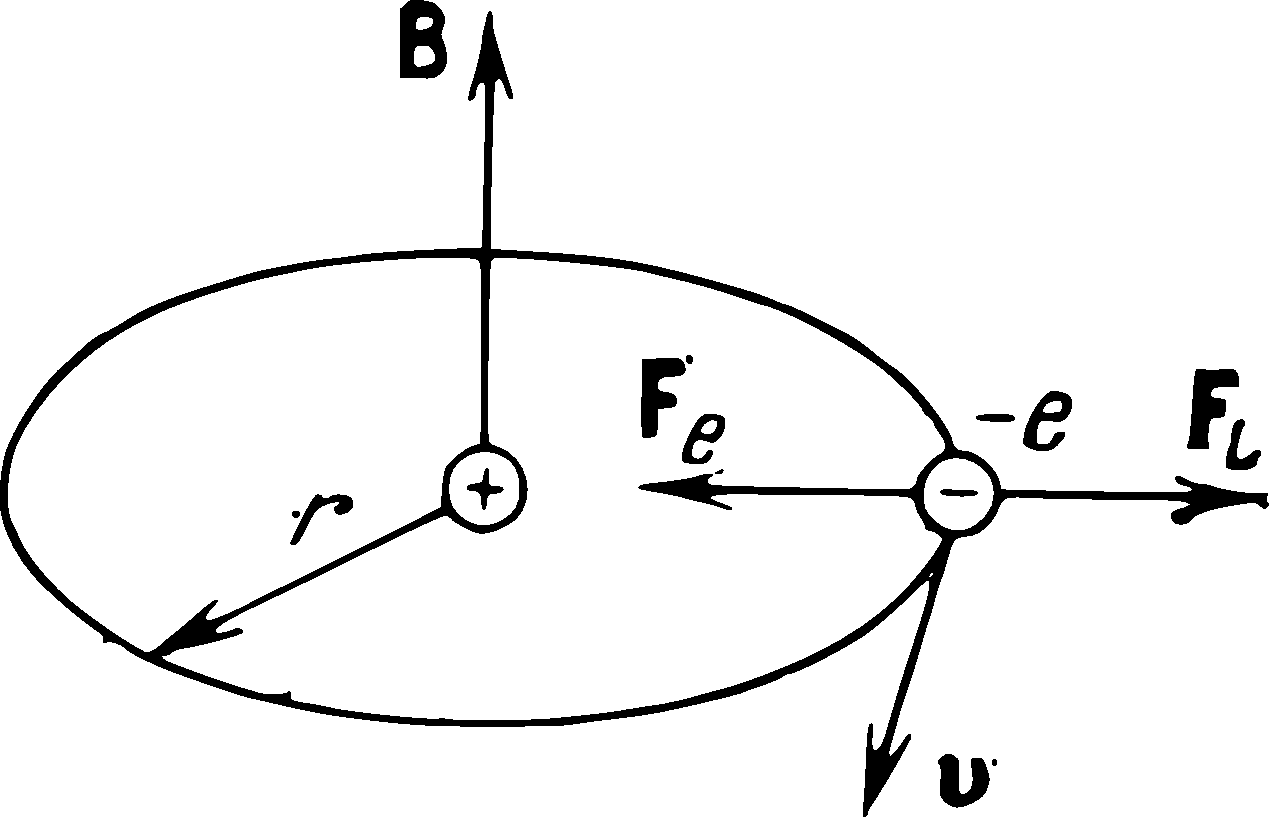
\includegraphics[width=0.8\textwidth]{figs/ch-26/fig-26-02.pdf}
\sidecaption{Forces on the electron.\zhcap{作用于电子上的力。}\label{fig-26-02}}
\end{marginfigure}

\subsection{}\label{26.2.2} The change in the angular velocity of the electron occurs in the process of growth of the magnetic field into which the atom is placed. This growth takes place during a finite length of time. At this an induced rotational electric field \ssect{25.1.1} is developed that acts on the electron in the atom. The strength $\vb{E}$ of this field is directed along a tangent to the electron's orbit and the force acting on the electron is $\vb{F} = e \vb{E}$ \ssect{15.1.2}. 
\zhpar{电子角速度的这种变化，发生在原子所处磁场增强的过程中。这一增强过程需要经历有限的时间。在此过程中产生的感生涡旋电场 \ssect{25.1.1} 作用于原子中的电子。该电场强度 $\vb{E}$ 沿电子轨道的切线方向，作用于电子的力为 $\vb{F} = e \vb{E}$ \ssect{15.1.2}。}

\subsection{}\label{26.2.3} Upon an arbitrary position of the electron's orbit with respect to vector $\vb{B}$, the orbital magnetic moment pm of the electron \ssect{26.1.2}) makes an angle $\alpha$ with the direction of the magnetic field (Fig. 26.3). In this case there will be a precessional motion of the orbit about the direction of vector $\vb{B}$ (\ssect{4.3.2}). This means that vector $\vb{p}_{m}$, perpendicular to the orbit and maintaining its angle $\alpha$ with the field constant, rotates about the direction, of vector $\vb{B}$ with the angular velocity $\omega_{L}$. Thus
\zhpar{当电子轨道相对于矢量 $\vb{B}$ 处于任意位置时，电子的轨道磁矩 $\vb{p}_{m}$（\ssect{26.1.2}）与磁场方向成夹角 $\alpha$（见图 26.3）。此时轨道将绕 $\vb{B}$ 的方向进动 \ssect{4.3.2}。这意味着，垂直于轨道的矢量 $\vb{p}_{m}$ 保持与磁场的夹角 $\alpha$ 不变，并以角速度 $\omega_{L}$ 绕 $\vb{B}$ 的方向旋转。于是有：}
\begin{align*}%
\omega_{L} & =  \frac{e B}{2m} && \text{(in SI units),} \\
\omega_{L} & =  \frac{e B}{2mc} && \text{(in Gaussian units)},
\end{align*}
Here $e$ is the magnitude of the charge of the electron, $m$ is its mass, $H$ is the magnetic field strength, $c$ is the electrodynamic constant \ssect{23.2.2}, and $\omega_{L}$ is called the \redem{angular velocity of Larmor precession}.
\zhpar{式中 $e$ 为电子电荷的绝对值，$m$ 为其质量，$H$ 为磁场强度，$c$ 为电动力学常量 \ssect{23.2.2}，$\omega_{L}$ 称为\redem{拉莫尔进动角速度}。}

Larmor's theorem states that the only result of the effect of a magnetic field on an electron's orbit in an atom is the precession
(in SI units),  of the orbit and vector $\vb{p}_{m}$ with the angular velocity $\omega_{L}$, about an axis through the nucleus of the atom and parallel to the induction vector $\vb{B}$ of the magnetic field.
\zhpar{拉莫尔定理指出，磁场对原子中电子轨道的唯一作用，是使轨道及矢量 $\vb{p}_{m}$ 以角速度 $\omega_{L}$ 绕通过原子核且平行于磁感应强度矢量 $\vb{B}$ 的轴线进动。}

\subsection{}\label{26.2.4} The precessional motion of the electron's orbit results in an additional orbital current $\Delta \, I_{orb}$ (\figr{fig-26-03}) and the corresponding induced orbital magnetic moment $\Delta \, \vb{p}_{m}$ \ssect{26.1.2} with the magnitude
\zhpar{电子轨道的进动产生附加轨道电流 $\Delta \, I_{orb}$（见\figr{fig-26-03}），并产生相应的感生轨道磁矩 $\Delta \, \vb{p}_{m}$ \ssect{26.1.2}，其大小为：}
\begin{align*}%
\Delta \, p_{m} & =  \Delta \, I_{orb} S_{\perp} = \frac{e^{2} S_{\perp}}{4 \pi m} && \text{(in SI units),} \\
\Delta \, p_{m} & =  \frac{1}{c} \Delta \, I_{orb} S_{\perp} = \frac{e^{2} S_{\perp}}{4 \pi m c^{2}} && \text{(in Gaussian units)},
\end{align*}
where $S_{\perp}$ is the area of the projection of the orbit on a plane perpendicular to the direction of vector $\vb{B}$. 
\zhpar{式中 $S_{\perp}$ 为轨道在垂直于磁感应强度矢量 $\vb{B}$ 方向的平面上的投影面积。}

\begin{figure}[h]%[-2cm]
\centering
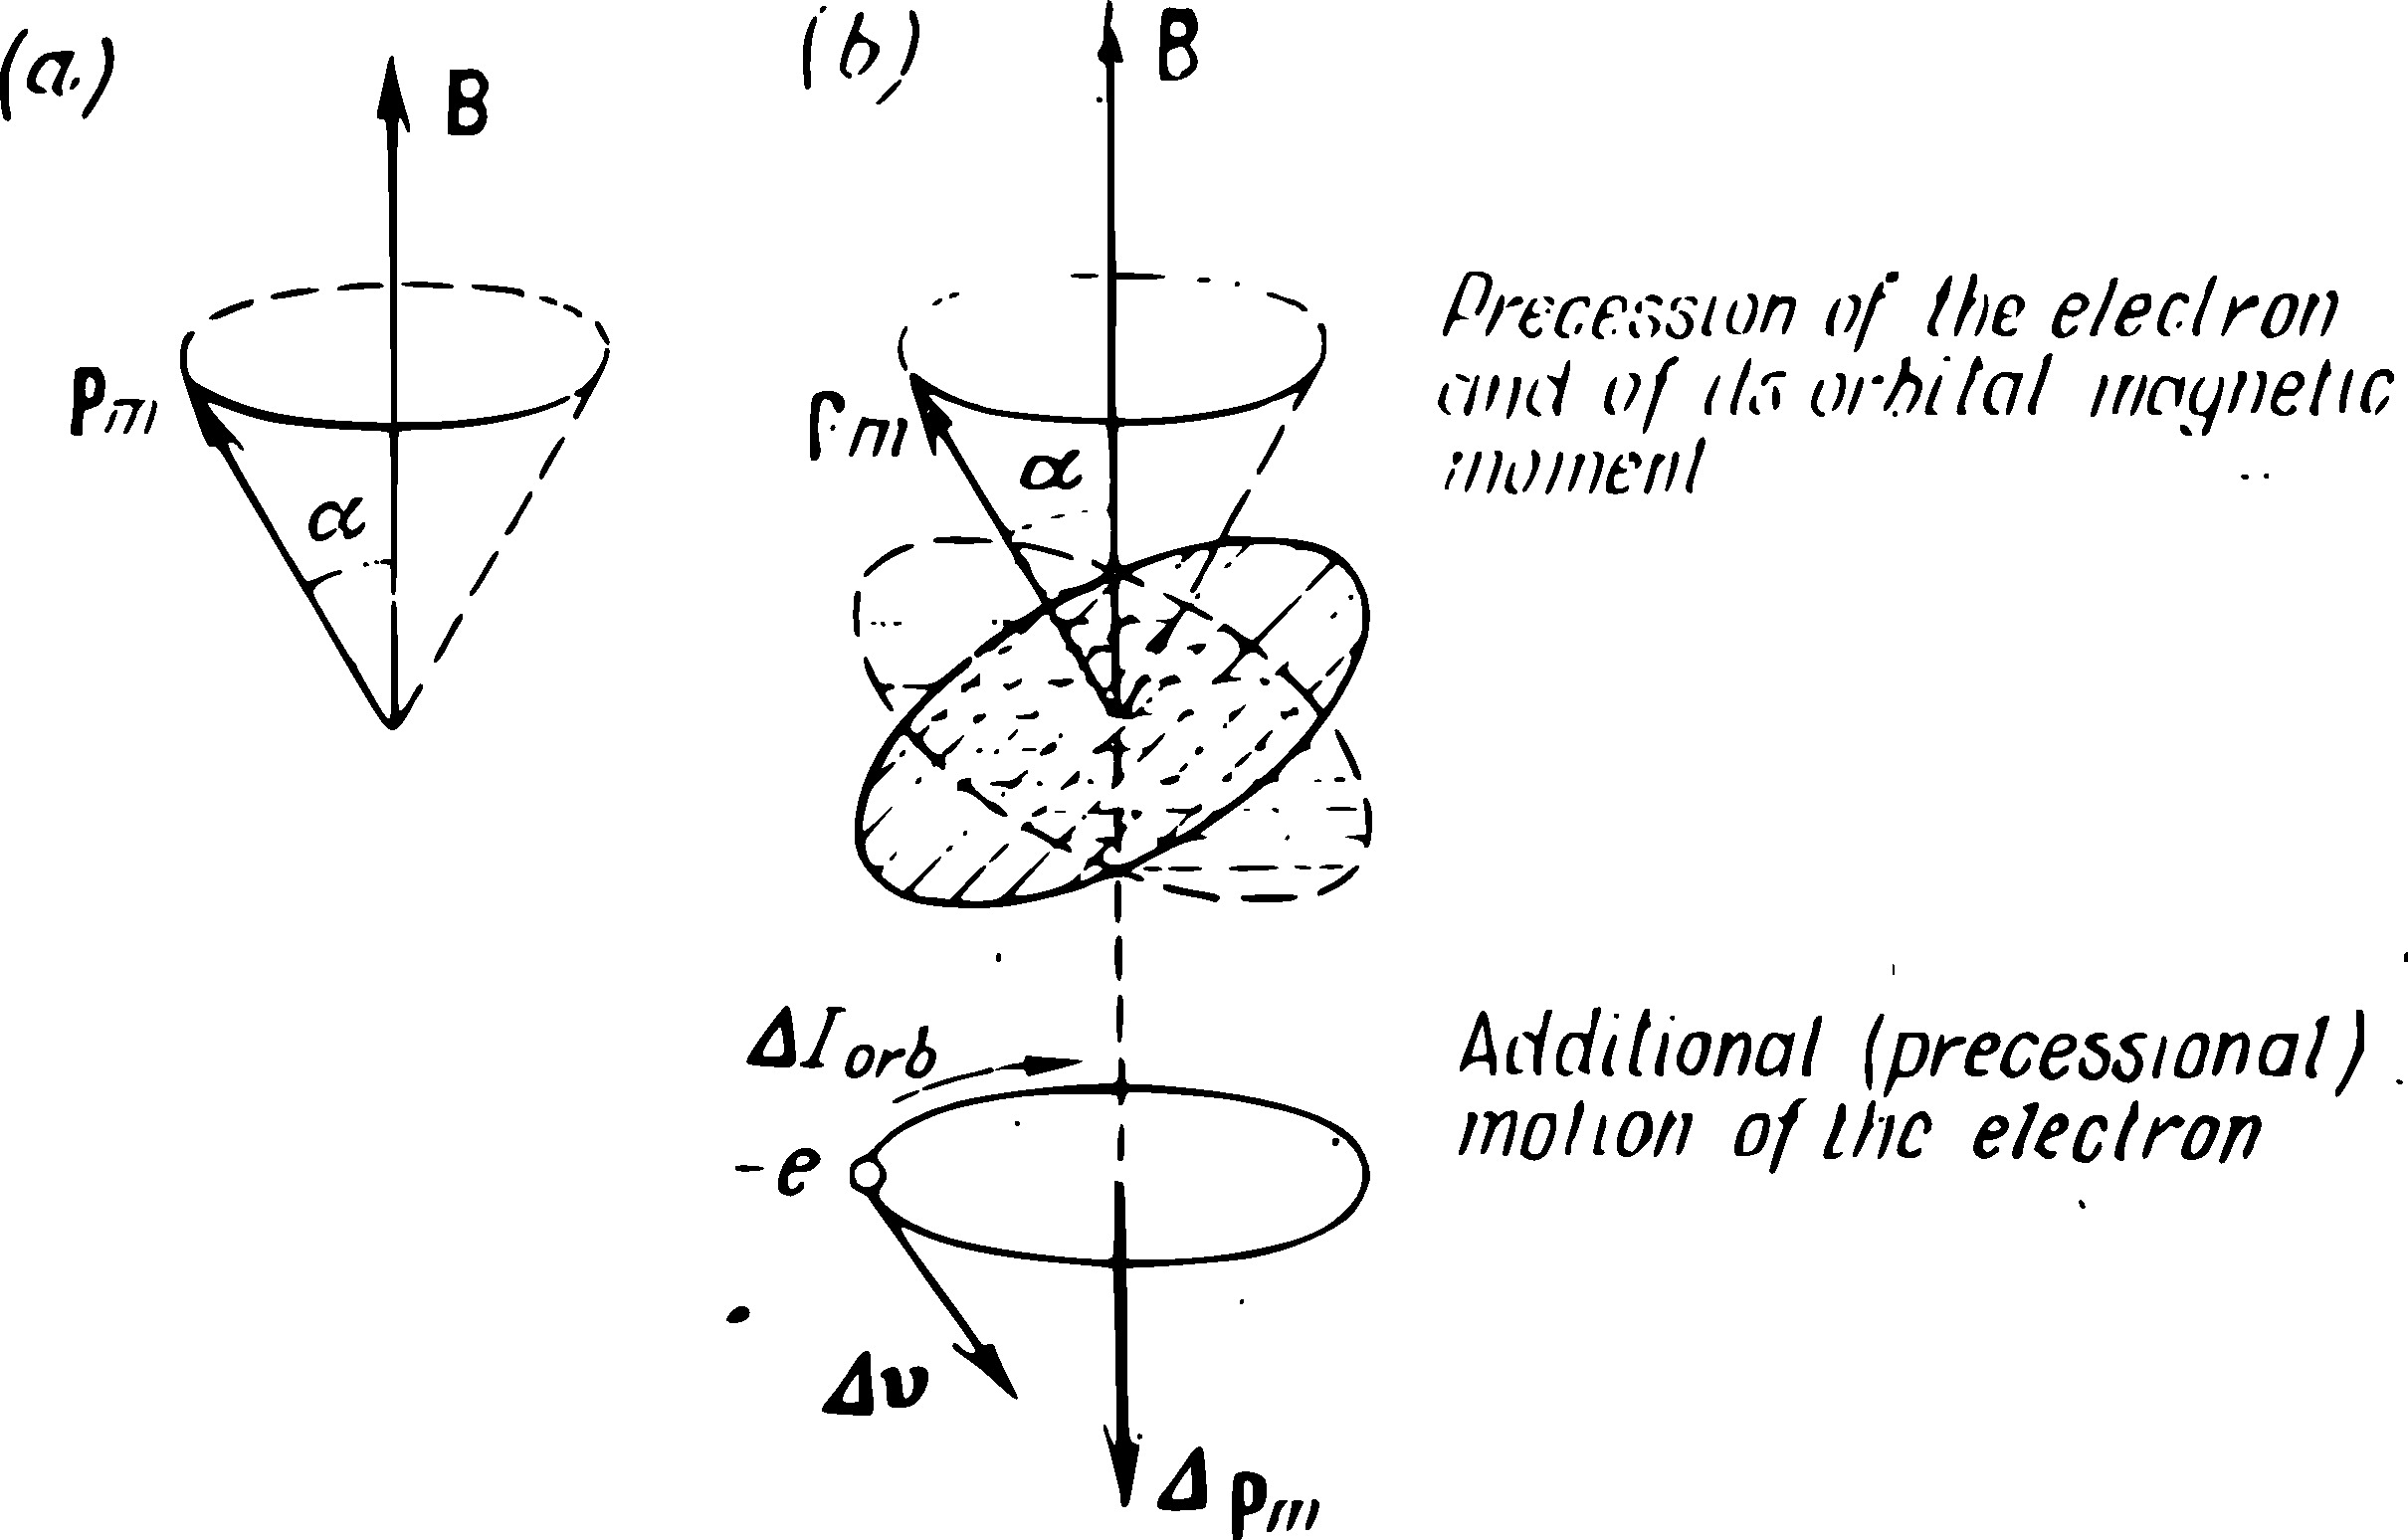
\includegraphics[width=\textwidth]{figs/ch-26/fig-26-03.pdf}
\sidecaption{Precession of the electron.\zhcap{电子的进动。}\label{fig-26-03}}
\end{figure}


Vector $\Delta \vb{p}_{m}$ has the direction opposite to the magnetic induction vector $\vb{B}$. Thus
\zhpar{矢量 $\Delta \vb{p}_{m}$ 的方向与磁感应强度矢量 $\vb{B}$ 相反。于是有：}
\begin{align*}%
\Delta \, \vb{p}_{m} & =  -\frac{e^{2} S_{\perp}}{4 \pi m} \vb{B}&& \text{(in SI units),} \\
\Delta \, \vb{p}_{m} & =  -\frac{e^{2} S_{\perp}}{4 \pi m c^{2}} \vb{B} && \text{(in Gaussian units)},
\end{align*}
The notation is the same as in \ssect{26.2.3}.
\zhpar{符号的含义与 \ssect{26.2.3} 中相同。}

The total induced orbital moment $\Delta \vb{P}_{m}$ of the atom \ssect{26.1.5}
\zhpar{原子的总感生轨道磁矩 $\Delta \vb{P}_{m}$（\ssect{26.1.5}）为：}
\begin{align*}%
\Delta \, \vb{P}_{m} & =  -\frac{e^{2}Z \expval{S_{\perp}}}{4 \pi m} \vb{B}&& \text{(in SI units),} \\
\Delta \, \vb{P}_{m} & =  -\frac{e^{2}Z \expval{S_{\perp}}}{4 \pi m c^{2}} \vb{B} && \text{(in Gaussian units)},
\end{align*}
where $Z$ is the number of electrons in the atom, and $\expval{S_{\perp}} = \sum_{i=1}^{z} S_{\perp \, i} /Z$ is the average area of the projections of the electron orbits on a plane perpendicular to the direction of vector $\vb{B}$.
\zhpar{式中 $Z$ 为原子中的电子数，$\expval{S_{\perp}} = \sum_{i=1}^{z} S_{\perp \, i} /Z$ 为电子轨道在垂直于 $\vb{B}$ 方向的平面上的投影面积的平均值。}

\section[Magnetic Materials in a Magnetic Field]{Diamagnetic and Paramagnetic Materials in a Uniform Magnetic Field
}
\label{sec-26.3}
\zhtitle{均匀磁场中的抗磁性与顺磁性物质}

\subsection{}\label{26.3.1} The magnetization of matter is characterized by the \redem{magnetization vector} (\redem{magnetization intensity}) $\vb{M}$, which is the ratio of the magnetic moment of a small volume $\Delta V$ of the substance to the magnitude of this volume. Thus
\zhpar{物质的磁化状态由\redem{磁化强度矢量}（\redem{磁化强度}）$\vb{M}$ 来描述，它等于物质中一小体积 $\Delta V$ 的磁矩与该体积大小之比。于是有：}
\begin{equation*}%
\vb{M} = \frac{1}{\Delta V} \sum_{i =1}^{N} \vb{P}_{m\,i}
\end{equation*}
where $\vb{P}_{m\,i}$ is the magnetic moment of the $i$-th atom (or molecule), and $N$ is the total number of atoms (or molecules) in the small volume $\Delta V$. Within the limits of the volume $\Delta V$ the magnetic field is assumed uniform. This volume should simultaneously contain a sufficiently large number of particles $N$ (i.e. $N \gg 1$) to enable the physical quantities characterizing the system of particles to be expediently averaged.
\zhpar{式中 $\vb{P}_{m\,i}$ 为第 $i$ 个原子（或分子）的磁矩，$N$ 为小体积 $\Delta V$ 内原子（或分子）的总数。在体积 $\Delta V$ 内，磁场被视为均匀的。该体积应同时包含足够多的粒子数 $N$（即 $N \gg 1$），以便对表征粒子系统的物理量进行方便的平均。}

\subsection{}\label{26.3.2} \redem{Diamagnetic materials} are substances in which the magnetic moments of the atoms (or molecules) equal zero in the absence of an external magnetic field. This means that in diamagnetic materials the vector sum of the orbital magnetic moments of all the electrons in an atom equals zero \ssect{26.1.5} and that induced magnetic moments \ssect{26.2.4} exist only in a magnetic field.
\zhpar{\redem{抗磁性物质}是指在没有外磁场时，其原子（或分子）的磁矩为零的物质。这意味着在抗磁性物质中，原子内所有电子的轨道磁矩的矢量和为零 \ssect{26.1.5}，而感生磁矩 \ssect{26.2.4} 只在磁场中存在。}

\subsection{}\label{26.3.3} In the volume $\Delta V$ of an isotropic diamagnetic material, the induced magnetic moments $\Delta \vb{}_{m}$ of all the atoms (or molecules) are the same and are opposite in direction to vector $\vb{B}$ \ssect{26.2.4}.
\zhpar{在各向同性抗磁性物质的体积 $\Delta V$ 内，所有原子（或分子）的感生磁矩 $\Delta \vb{}_{m}$ 都相同，且方向与矢量 $\vb{B}$ 相反 \ssect{26.2.4}。}

The magnetization vector $\vb{M}$ is equal to 
\zhpar{磁化强度矢量 $\vb{M}$ 等于：}
\begin{equation*}%
\vb{M} = \frac{N \Delta \vb{P}_{m}}{\Delta V}= n_{0} \vb{P}_{m},
\end{equation*}
and, taking \ssect{26.2.4} into account:
\zhpar{并考虑 \ssect{26.2.4}，有：}
\begin{align*}%
\vb{M} & =  -\frac{n_{0} e^{2} Z \expval{S_{\perp}}}{4 \pi m} \, \vb{B}&& \text{(in SI units),} \\
\vb{M} & =  -\frac{n_{0} e^{2} Z \expval{S_{\perp}}}{4 \pi mc^{2}} \,  \vb{B} && \text{(in Gaussian units)},
\end{align*}
where $n_{0}$ is the number of atoms (or molecules) in unit volume. The other notation is the same as in \ssect{26.2.4}. Introducing the notation:
\zhpar{式中 $n_{0}$ 为单位体积内的原子（或分子）数，其余符号与 \ssect{26.2.4} 中相同。引入记号：}
\begin{align*}%
\chi_{m}' & =  -\frac{n_{0} e^{2} Z \expval{S_{\perp}}\mu_{0}}{4 \pi m} && \text{(in SI units),} \\
\chi_{m}' & =  -\frac{n_{0} e^{2} Z \expval{S_{\perp}}}{4 \pi mc^{2}} && \text{(in Gaussian units)},
\end{align*}
we have g
\zhpar{于是有：}
\begin{align*}%
\vb{M} & =  \chi_{m}' \frac{\vb{B}}{\mu_{0}} && \text{(in SI units),} \\
\vb{M} & =  \chi_{m}' {\vb{B}}  && \text{(in Gaussian units)},
\end{align*}
where $\chi_{m}'$ is a dimensionless quantity that characterizes the magnetic properties of magnetic materials. For all diamagnetic
materials $\chi_{m}' < 0$.
\zhpar{式中 $\chi_{m}'$ 为表征磁性材料磁性质的无量纲量。对于所有抗磁性物质，$\chi_{m}' < 0$。}

\subsection{}\label{26.3.4} The \redem{magnetic susceptibility} $\chi_{m}$ is a quantity that is re­lated to $\chi_{m}'$ as follows:
\zhpar{\redem{磁化率} $\chi_{m}$ 与 $\chi_{m}'$ 的关系如下：}
\begin{align*}%
1 + \chi_{m} & =  \frac{1}{1 - \chi_{m}'} && \text{(in SI units),} \\
1 + 4\pi \, \chi_{m} & =  \frac{1}{1 - 4 \pi \,\chi_{m}'}  && \text{(in Gaussian units)},
\end{align*}
from which
\zhpar{由此得：}
\begin{align*}%
\chi_{m} & =  \frac{\chi_{m}'}{1 - \chi_{m}'} && \text{(in SI units),} \\
\chi_{m} & =  \frac{\chi_{m}'}{1 - 4\pi \, \chi_{m}'} && \text{(in Gaussian units)},
\end{align*}
Practically, $\chi_{m} = \chi_{m}'$ for diamagnetic materials, because in absolute value $\chi_{m}'$ is very small: $\abs{\chi_{m}'} \approx  \num{d-6}$.
\zhpar{因此，对于抗磁性物质，$\chi_{m} = \chi_{m}'$，这是因为 $\chi_{m}'$ 的绝对值很小：$\abs{\chi_{m}'} \approx \num{d-6}$。}

\subsection{}\label{26.3.5} \redem{Paramagnetic materials} are substances in which the atoms (or molecules) have a certain constant magnetic moment $\vb{P}_{m}$ in the absence of an external magnetic field. This means that the vector sum of the orbital magnetic moments of all the electrons. of an atom (or. molecule) is not equal to zero \ssect{26.1.5}.
\zhpar{\redem{顺磁性物质}是指在没有外磁场时，其原子（或分子）具有一定恒定磁矩 $\vb{P}_{m}$ 的物质。这意味着原子（或分子）内所有电子的轨道磁矩的矢量和不为零 \ssect{26.1.5}。}

\subsection{}\label{26.3.6} When a paramagnetic material is placed into a uniform magnetic field \ssect{23.1.3}, the constant magnetic moments of the atoms (or molecules) precess about the direction of the induction vector $\vb{B}$ of the magnetic field at Larmor's angular velocity $\omega_{L}$ \ssect{26.2.3}.
\zhpar{将顺磁性物质置于均匀磁场 \ssect{23.1.3} 中时，原子（或分子）的恒定磁矩将以拉莫尔角速度 $\omega_{L}$（\ssect{26.2.3}）绕磁感应强度矢量 $\vb{B}$ 的方向进动。}

Thermal motion and collisions of the1atoms (or molecules) of a paramagnetic material lead to a gradual damping of the precession of the magnetic moments and to a reduction in the angles between the directions of the magnetic moment vectors and vector $\vb{B}$. The combined actions of the interatomic collisions and the magnetic field lead to a predominant orientation of the magnetic moments of the atoms in alignment with the external field. 
\zhpar{顺磁性物质中原子（或分子）的热运动和相互碰撞，使磁矩的进动逐渐衰减，并使磁矩矢量与矢量 $\vb{B}$ 之间的夹角减小。原子间碰撞与磁场的共同作用，使原子磁矩主要沿外磁场方向取向。}

Though the constant magnetic moment $\vb{P}_{m}$ of an atom (or molecule) is of the order of \SI{d-23}{\joule\per\tesla} (\SI{d-20}{\erg\per\gauss}, the magnetic moments of all the particles in unit volume produce a magnetization that considerably exceeds diamagnetic phenomena \ssect{26.3.3}. A paramagnetic material in an external magnetic field has an intrinsic magnetic field aligned with the external magnetic field.
\zhpar{尽管原子（或分子）的恒定磁矩 $\vb{P}_{m}$ 的量级仅为 \SI{d-23}{\joule\per\tesla}（即 \SI{d-20}{\erg\per\gauss}），但单位体积内所有粒子的磁矩所产生的磁化强度，远超过抗磁性现象 \ssect{26.3.3}。处于外磁场中的顺磁性物质，具有与外磁场方向一致的内禀磁场。}

\subsection{}\label{26.3.7} In the classical theory of paramagnetism the magnitude of the magnetization vector \ssect{26.3.1} is expressed by the formula
\zhpar{在顺磁性的经典理论中，磁化强度矢量的大小（\ssect{26.3.1}）由下式表示：}
\begin{equation*}%
M= n_{0} P_{m} L(a),
\end{equation*}
where $n_{0}$ is the number of atoms (or molecules) in unit volume, and $L (a)$ is the classical Langevin function:
\zhpar{式中 $n_{0}$ 为单位体积内的原子（或分子）数，$L (a)$ 为经典\redem{朗之万函数}：}
\begin{equation*}%
L(a) = \frac{e^{a} + e^{-a}}{e^{a}-e^{-a}} - \frac{1}{a}.
\end{equation*}
The parameter $a$ is of the form $a = P_{m}B/kT$, where $B$ is the magnetic induction of the field, $k$ is Boltzmann's constant \ssect{8.4.5}, and $T$ is the absolute temperature. At room temperature and not especially strong external fields, $a \ll 1$ and the function $L (a)$ is, simplified, after expansion into a a series, and we obtain $L (a) \approx a/3$. Hence, the magnetization vector, is equal to
\zhpar{参数 $a$ 的形式为 $a = P_{m}B/kT$，式中 $B$ 为磁场的磁感应强度，$k$ 为玻尔兹曼常量 \ssect{8.4.5}，$T$ 为热力学温度。在室温且外场不太强的情况下，$a \ll 1$，将函数 $L (a)$ 展开成级数并作简化，得 $L (a) \approx a/3$。于是，磁化强度矢量等于：}
\begin{align*}%
\vb{M} & = \chi_{m}' \frac{\vb{B}}{\mu_{0}} && \text{(in SI units),} \\
\vb{M} & = \chi_{m}' \vb{B} && \text{(in Gaussian units)},
\end{align*}
where $\chi_{m}'$ is determined by the formula
\zhpar{式中 $\chi_{m}'$ 由下式确定：}
\begin{align*}%
\chi_{m}' & =  \frac{n_{0}P_{m}^{2}\mu_{0}}{3kT} && \text{(in SI units),} \\
\chi_{m}' & =  \frac{n_{0}P_{m}^{2}}{3kT} && \text{(in Gaussian units)}.
\end{align*}
The quantity $\chi_{m}'$ is related to the magnetic susceptibility $\chi_{m}$ of paramagnetic materials by the formulas given in \ssect{26.3.4}.
\zhpar{量 $\chi_{m}'$ 与顺磁性物质的磁化率 $\chi_{m}$ 之间的关系，由 \ssect{26.3.4} 中给出的公式确定。}

The value of the quantity $\chi_{m}$ is positive for a paramagnetic
material and ranges from \num{d-5} to \num{d-3}; therefore, $\chi_{m}' = \chi_{m}$ with a high degree of accuracy.
\zhpar{顺磁性物质的磁化率 $\chi_{m}$ 为正值，其数值范围为 \num{d-5} 至 \num{d-3}；因此，$\chi_{m}' = \chi_{m}$ 具有很高的精确度。}

The \redem{Curie law} states that the paramagnetic susceptibility of a substance is inversely proportional to the absolute tempera­ ture.
\zhpar{\redem{居里定律}指出，物质的顺磁性磁化率与热力学温度成反比。}

\subsection{}\label{26.3.8} In very strong external magnetic fields, saturation magnetization is reached; here $a \gg 1$ and the Langevin function $L (a) \to  1$. This means that the magnetic moments of all the atoms (or molecules) are aligned with the external magnetic field and $M = n_{0}P_{m}$.
\zhpar{在极强的外磁场中，达到饱和磁化。此时 $a \gg 1$，朗之万函数 $L (a) \to 1$。这意味着所有原子（或分子）的磁矩都与外磁场方向一致，且 $M = n_{0}P_{m}$。}

\section{Magnetic Field in Magnetic Materials}
\label{sec-26.4} 
\zhtitle{磁性材料中的磁场}

\subsection{}\label{26.4.1} Two types of currents that set up magnetic fields, macrocurrents and microcurrents, can be distinguished in matter. What we have called \redem{macrocurrents} here are conduction currents \ssect{20.1.2} and convection currents \ssect{20.1.2}. \redem{Microcurrents} (molecular currents) are those due to the motion of electrons in atoms, molecules and ions.
\zhpar{物质中可以区分出两类产生磁场的电流：宏观电流和微观电流。这里所称的\redem{宏观电流}，是指传导电流 \ssect{20.1.2} 和运流电流 \ssect{20.1.2}。\redem{微观电流}（分子电流）则是由原子、分子和离子中电子的运动所产生的电流。}

The magnetic field in a substance is the vector sum of two fields \ssect{15.2.2}: the \redem{external} magnetic field, set up by the macrocurrents, and the \redem{internal}, or \redem{intrinsic magnetic field}, set up by microcurrents. The magnetic induction vector $\vb{B}$ \ssect{23.1.2} in the magnetic field in a substance characterizes the resultant magnetic field and is equal to the vector sum of the magnetic inductions of the external $\vb{B}_{0}$ and intrinsic $\vb{B}_{intr}$ magnetic fields. Thus
\zhpar{物质中的磁场是两个磁场的矢量和 \ssect{15.2.2}：一个是由宏观电流建立的\redem{外磁场}，另一个是由微观电流建立的\redem{内禀磁场}（或称\redem{固有磁场}）。物质中磁场的磁感应强度矢量 $\vb{B}$ \ssect{23.1.2} 表征合成磁场，它等于外磁场的磁感应强度 $\vb{B}_{0}$ 与内禀磁场的磁感应强度 $\vb{B}_{intr}$ 的矢量和。于是有：}
\begin{equation*}%
\vb{B} = \vb{B}_{0} + \vb{B}_{intr}
\end{equation*}
The primary source of magnetic fields in magnetic materials are the macrocurrents. Their magnetic fields are what leads to the magnetization of substances placed in an external magnetic field.
\zhpar{磁性材料中磁场的主要来源是宏观电流。正是它们产生的磁场，导致置于外磁场中的物质被磁化。}

\subsection{}\label{26.4.2} The \redem{total current law for a magnetic field in a substance} is a generalization of the law formulated in \ssect{23.5.2}:
\zhpar{\redem{磁场在物质中的全电流定律}是 \ssect{23.5.2} 中所述定律的推广：}
\begin{align*}%
\oint_{L} \vb{B} \, \dd \vb{l} & =  \mu_{0} (I_{mic} + I_{mac}) && \text{(in SI units),} \\
\oint_{L} \vb{B} \, \dd \vb{l} & = \frac{4\pi}{c} \mu_{0} (I_{mic} + I_{mac}) && \text{(in Gaussian units)}.
\end{align*}
where $I_{mac}$ and $I_{mic}$ are the algebraic sums of the macro- and microcurrents passing through a surface bounded by the loop $L$. 
\zhpar{式中 $I_{mac}$ 与 $I_{mic}$ 分别为穿过以回路 $L$ 为边界的曲面的宏观电流与微观电流的代数和。}

\subsection{}\label{26.4.3} The algebraic sum of the microcurrents is related to the magnetization vector $\vb{M}$ as follows:
\zhpar{微观电流的代数和与磁化强度矢量 $\vb{M}$ 的关系如下：}
\begin{align*}%
I_{mic} & =  \oint_{L} \vb{M} \, \dd \vb{l} && \text{(in SI units),} \\
I_{mic} & =  c \oint_{L} \vb{M} \, \dd \vb{l} && \text{(in Gaussian units)},
\end{align*}
where $\oint \vb{M} \, \dd \vb{l}$ is the circulation of the magnetization vector $\vb{M}$ \ssect{26.3.1} along the closed loop $L$ through which the microcurrents are threaded.
\zhpar{式中 $\oint \vb{M} \, \dd \vb{l}$ 为磁化强度矢量 $\vb{M}$（\ssect{26.3.1}）沿闭合回路 $L$ 的环流，微观电流穿过该闭合回路。}

The final form of the total current law \ssect{26.4.2} is
\zhpar{全电流定律 \ssect{26.4.2} 的最终形式为：}
\begin{align*}%
\oint_{L} \left(\frac{\vb{B}}{\mu_{0}} - \vb{M} \right) \, \dd \vb{l} & =  I_{mac} && \text{(in SI units),} \\
\oint_{L} \left(\vb{B} - 4\pi \vb{M} \right) \, \dd \vb{l} & =  \frac{4\pi}{c} I_{mac} && \text{(in Gaussian units)}.
\end{align*}

\subsection{}\label{26.4.4}

The vector
\zhpar{矢量}
\begin{align*}%
\vb{H} & = \frac{\vb{B}}{\mu_{0}} - \vb{M} && \text{(in SI units),} \\
\vb{H} & = \vb{B} - 4 \pi \vb{M} && \text{(in Gaussian units)}.
\end{align*}
is called the \redem{strength of the magnetic field} existing in an arbitrary medium (cf. \ssect{23.2.3}). The total current, law for a magnetic field in an arbitrary medium is written in a form identical to that in \ssect{23.5.4}:
\zhpar{称为任意介质中存在的\redem{磁场强度}（参见 \ssect{23.2.3}）。任意介质中磁场的全电流定律，其形式与 \ssect{23.5.4} 中的形式完全相同：}
\begin{align*}%
\oint_{L} \vb{H} \, \dd \vb{l} & =  I_{mac} && \text{(in SI units),} \\
\oint_{L} \vb{H} \, \dd \vb{l} & =  \frac{4\pi}{c} I_{mac} && \text{(in Gaussian units)}.
\end{align*}
The circulation of the magnetic field strength vector along an arbitrary closed loop is equal (or proportional) to the algebraic sum of the macrocurrents through the surface hounded by this loop.
\zhpar{磁场强度矢量沿任意闭合回路的环流，等于（或正比于）穿过该回路所围曲面的宏观电流的代数和。}

\subsection{}\label{26.4.5} For an isotropic medium, the relation between the magnetic induction vector $\vb{B}$ and the magnetization vector $\vb{M}$ \ssect{26.3.1} leads to the following result for vector $\vb{H}$ \ssect{26.4.4}:
\zhpar{对于各向同性介质，磁感应强度矢量 $\vb{B}$ 与磁化强度矢量 $\vb{M}$（\ssect{26.3.1}）之间的关系，给出矢量 $\vb{H}$（\ssect{26.4.4}）的如下结果：}
\begin{align*}%
\vb{H} & =  (1 - \chi_{m}') \frac{\vb{B}}{\mu_{0}} && \text{(in SI units),} \\
\vb{H} & =  (1 - 4 \pi \chi_{m}') \vb{B} && \text{(in Gaussian units)}.
\end{align*}
Substituting for $(1 - \chi_{m}')$ or $(1 - 4\pi \chi_{m}')$ on the basis of Sect. 26.3.4, we have
\zhpar{利用 \ssect{26.3.4} 对 $(1 - \chi_{m}')$ 或 $(1 - 4\pi \chi_{m}')$ 进行代换，得：}
\begin{align*}%
\vb{H} & =   \frac{\vb{B}}{\mu_{0}\mu_{r}} && \text{(in SI units),} \\
\vb{H} & =  \frac{\vb{B}}{\mu_{r}} && \text{(in Gaussian units)}.
\end{align*}
where
\zhpar{式中：}
\begin{align*}%
\mu_{r} & =  1 + \chi_{m} && \text{(in SI units),} \\
\mu_{r} & =  1 + 4\pi \chi_{m}  && \text{(in Gaussian units)}.
\end{align*}
The quantity $\mu_{r}$ thus introduced is called the \redem{relative magnetic permeability} of the substance (see also \ssect{23.2.1}). In these formulas $\chi_{m}$ is the magnetic susceptibility \ssect{26.3.4}.
\zhpar{由此引入的量 $\mu_{r}$ 称为该物质的\redem{相对磁导率}（另见 \ssect{23.2.1}）。式中 $\chi_{m}$ 为磁化率 \ssect{26.3.4}。}


\section{Ferromagnetic Materials}
\label{sec-26.5} 
\zhtitle{铁磁性材料}

\subsection{}\label{26.5.1} \redem{Ferromagnetic materials} are substances in which the intrinsic (internal) magnetic field \ssect{26.4.1} is hundreds or even thousands of times stronger than the external magnetic field applied to the substance.
\zhpar{\redem{铁磁性物质}是指其内禀（内部）磁场 \ssect{26.4.1} 比施加于该物质的外磁场强数百甚至数千倍的物质。}

Ferromagnetism is observed in the crystals of the transition metals \ssect{39.3.8}, iron, cobalt and nickel and of certain alloys, provided that $d/a  \gg 1.5$, where $d$ is the diameter of the atom and $a$ is the diameter of the unfilled electronic shell of the atom \ssect{39.3.6}.
\zhpar{铁磁性见于过渡金属 \ssect{39.3.8}（铁、钴、镍）的晶体以及某些合金的晶体中，但需满足 $d/a \gg 1.5$，其中 $d$ 为原子的直径，$a$ 为原子中未填满电子壳层的直径 \ssect{39.3.6}。}


\begin{marginfigure}[-2.75cm]
\centering
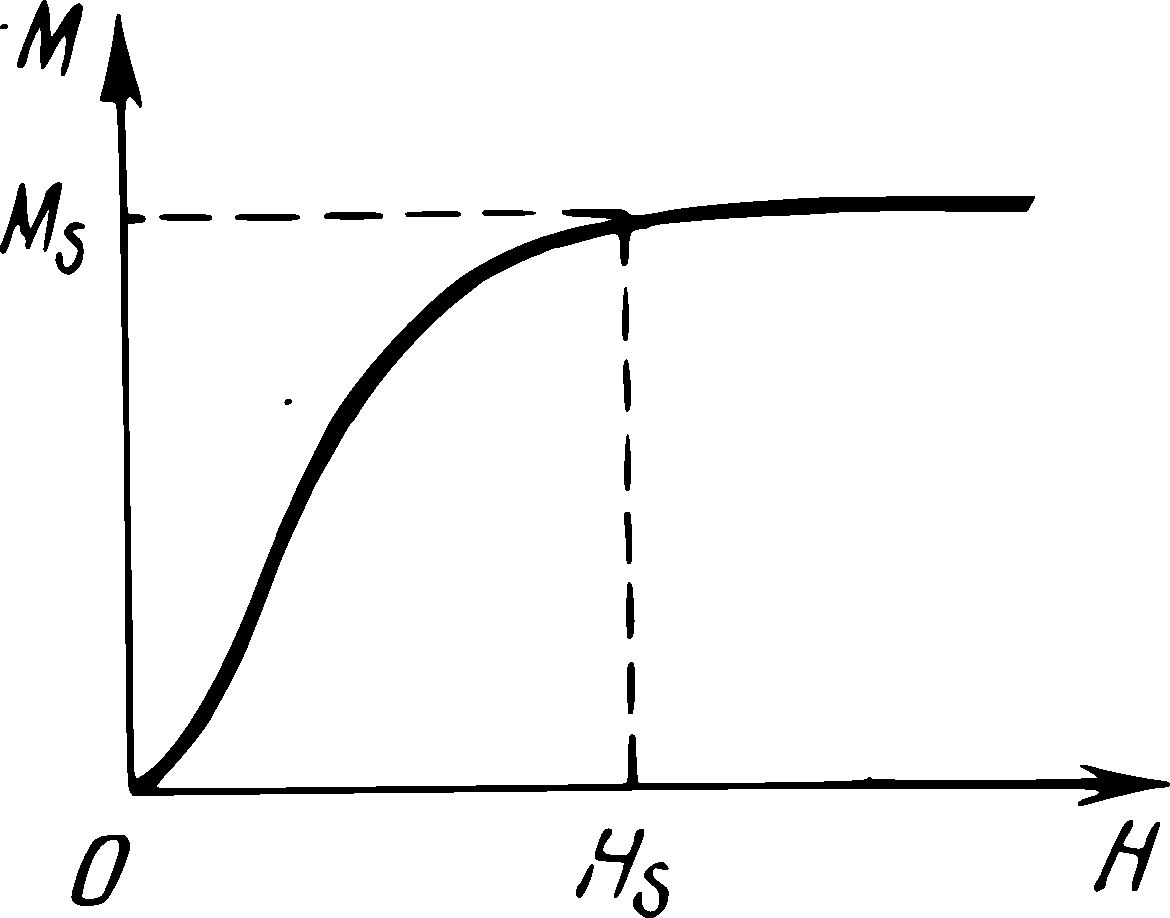
\includegraphics[width=0.8\textwidth]{figs/ch-26/fig-26-04.pdf}
\sidecaption{The dependence of the magnetization \ssect{26.3.1} on the strength $H$ of the external magnetic field and magnetic saturation $M_{s}$.\zhcap{磁化强度 \ssect{26.3.1} 随外磁场强度 $H$ 的变化关系，以及磁饱和值 $M_{s}$。}\label{fig-26-04}}
\end{marginfigure}


\subsection{}\label{26.5.2} The principal properties of ferromagnetic materials, distinguishing them from other magnetic materials are:
\zhpar{铁磁性物质区别于其他磁性材料的主要性质如下：}
\begin{enumerate}[label = (\alph*)]
\item The dependence of the magnetization \ssect{26.3.1} on the strength $H$ of the external magnetic field is characterized by \redem{magnetic saturation} $M_{s}$, which begins at $H \geqslant H_{s}$ (\figr{fig-26-04}).
\zhpar{磁化强度 \ssect{26.3.1} 随外磁场强度 $H$ 的变化关系，以\redem{磁饱和} $M_{s}$ 为特征，磁饱和始于 $H \geqslant H_{s}$（见\figr{fig-26-04}）。}
\item The dependence of the magnetic induction $\vb{B}$ on $\vb{H}$ is characterized by the increase according to a linear law at $H \geqslant H_{s}$ (\figr{fig-26-05}).
\zhpar{磁感应强度 $\vb{B}$ 随 $\vb{H}$ 的变化关系，以当 $H \geqslant H_{s}$ 时按线性规律增加为特征（见\figr{fig-26-05}）。}
\begin{marginfigure}[-2.75cm]
\centering
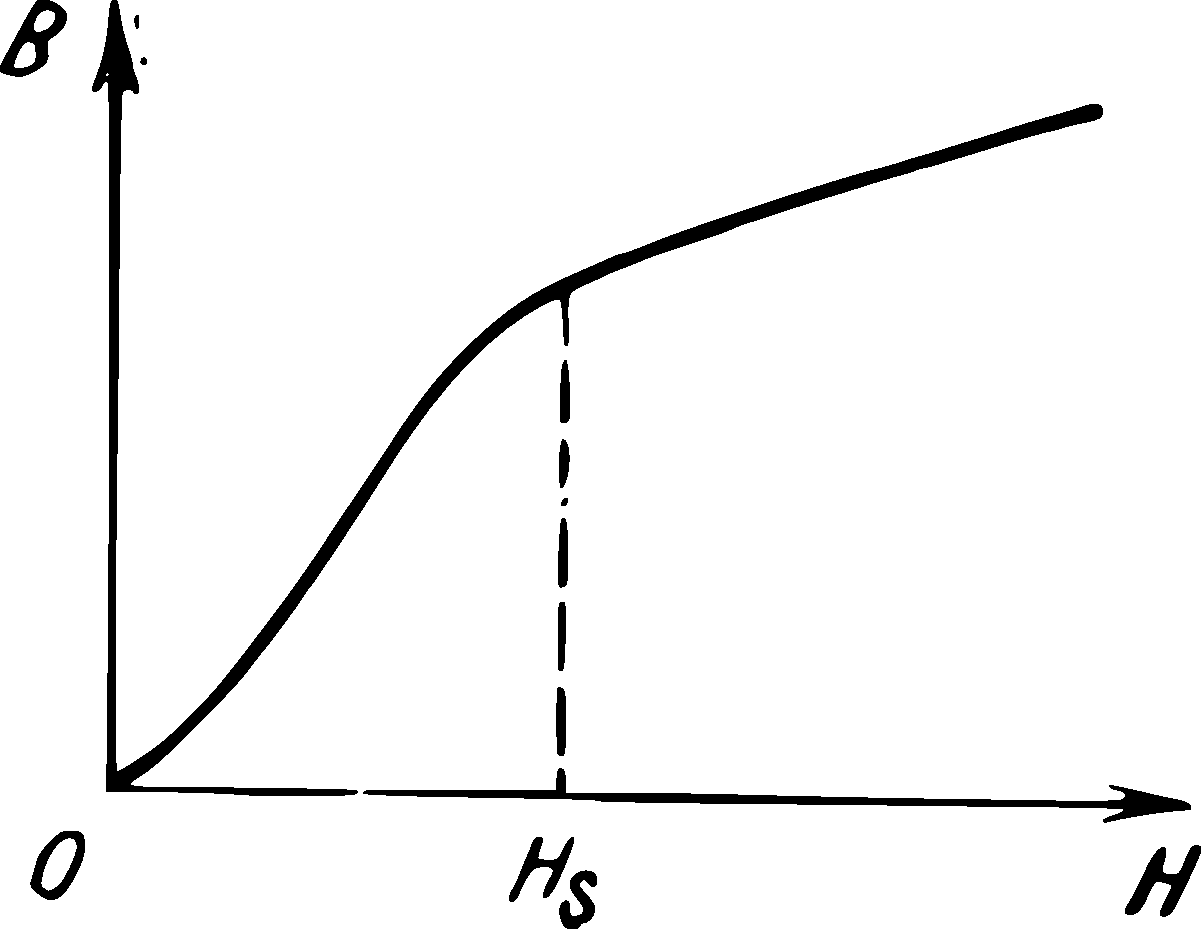
\includegraphics[width=0.8\textwidth]{figs/ch-26/fig-26-05.pdf}
\sidecaption{The dependence of the magnetic induction $\vb{B}$ on $\vb{H}$.\zhcap{磁感应强度 $\vb{B}$ 随 $\vb{H}$ 的变化关系。}\label{fig-26-05}}
\end{marginfigure}

\item The dependence of the relative magnetic permeability $\mu_{r}$ on the field strength $H$ is of a complex nature (\figr{fig-26-06}). 
\zhpar{相对磁导率 $\mu_{r}$ 随磁场强度 $H$ 的变化关系较为复杂（见\figr{fig-26-06}）。}
\item \redem{Magnetic hysteresis} exists in ferromagnetic materials. This refers to the lag in the variation of magnetization from the variation in the strength of the external magnetizing field, which is variable in magnitude and direction. This lag is due to the dependence of $M$ on its previous values (past history) in magnetizing the substance.
\zhpar{铁磁性物质中存在\redem{磁滞}现象。它是指当外磁化场的大小和方向变化时，磁化强度的变化落后于外磁场强度变化的现象。这种滞后是由于磁化过程中 $M$ 取决于其先前的数值（即历史过程）。}
\begin{marginfigure}[-3cm]
\centering
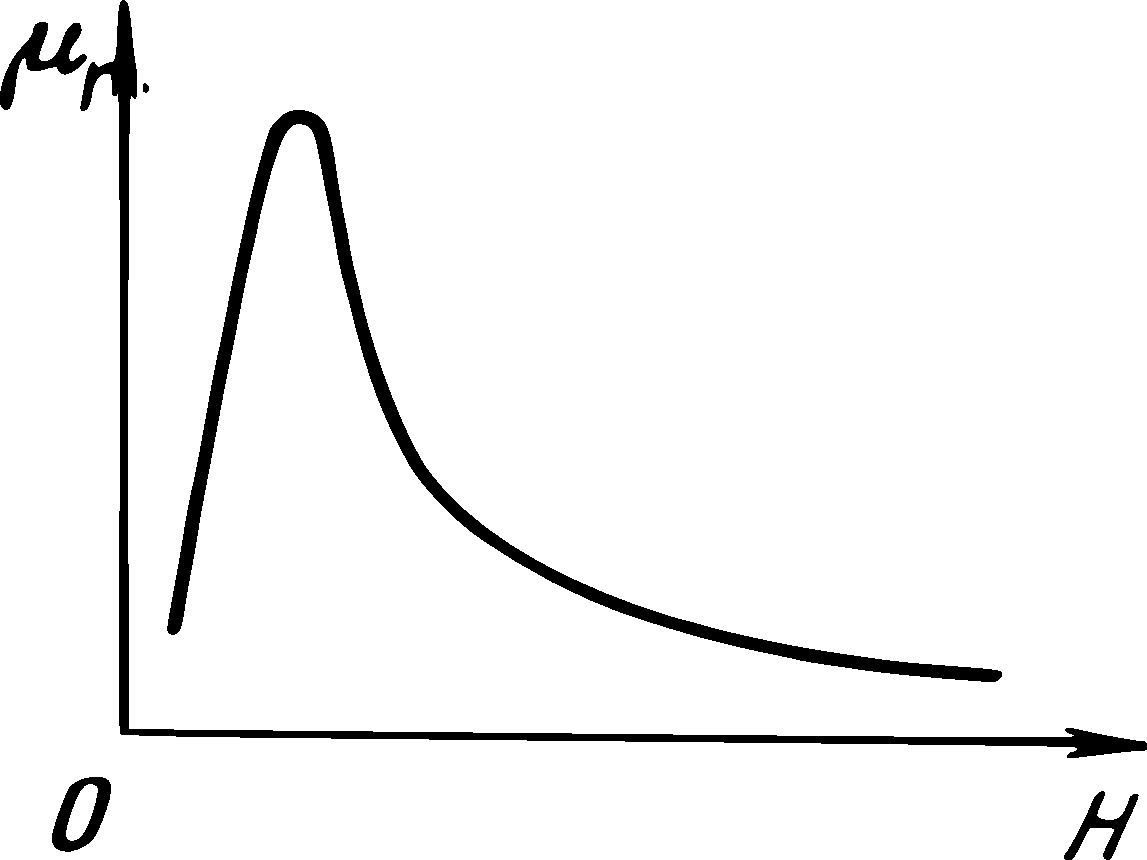
\includegraphics[width=0.8\textwidth]{figs/ch-26/fig-26-06.pdf}
\sidecaption{The dependence of the relative magnetic permeability $\mu_{r}$ on the field strength $H$.\zhcap{相对磁导率 $\mu_{r}$ 随磁场强度 $H$ 的变化关系。}\label{fig-26-06}}
\end{marginfigure}
\item The properties of ferromagnetic materials enumerated above\sidenote[][4cm]{As well as many others that are beyond the scope of this handbook.} are observed at temperatures below the \redem{Curie point} $\theta_{C}$ \ssect{18.4.4}. At temperatures $T \geqslant \theta_{C}$, thermal motion breaks up the regions of spontaneous magnetization \ssect{26.5.4} and the ferromagnetic material, losing its special features, is converted into a paramagnetic substance \ssect{26.3.5}. The Curie points for iron, nickel, cobalt and Permalloy are 1043, 631, 1403 and 823 K.
\zhpar{上述铁磁性物质的各项性质，均在低于\redem{居里点} $\theta_{C}$ \ssect{18.4.4} 的温度下观察到。当 $T \geqslant \theta_{C}$ 时，热运动破坏了自发磁化区 \ssect{26.5.4}，铁磁性物质失去其特殊性质，转变为顺磁性物质 \ssect{26.3.5}。铁、镍、钴和坡莫合金的居里点分别为 1043 K、631 K、1403 K 和 823 K。}
\zhpar{注：此外还有许多其他性质，超出了本手册的范围。}
\end{enumerate}



\subsection{}\label{26.5.3} The \redem{hysteresis loop} is a curve showing the change in the magnetization of a ferromagnetic material located in an external magnetic field as the strength of this field is varied from $+H_{s}$ to $-H_{s}$ and back again, where $H_{s}$ is the field strength corresponding to magnetic saturation (\figr{fig-26-07}). The magnetization $\pm M_{s}$ at $H = \pm H_{s}$ is called \redem{saturation magnetization}. The magnetization $\pm M_{r}$ that remains in a ferromagnetic material in the absence of an external field $(H = 0)$ is called the \redem{residual}, or \redem{remanent, magnetization}. This factor is the basis for making permanent magnets. 
\zhpar{\redem{磁滞回线}是表示位于外磁场中的铁磁性物质，其磁化强度随外磁场强度从 $+H_{s}$ 变至 $-H_{s}$ 再返回时变化的曲线，其中 $H_{s}$ 为对应磁饱和的磁场强度（见\figr{fig-26-07}）。在 $H = \pm H_{s}$ 时的磁化强度 $\pm M_{s}$ 称为\redem{饱和磁化强度}。在没有外场（$H = 0$）时，铁磁性物质中保留的磁化强度 $\pm M_{r}$ 称为\redem{剩余磁化强度}，或称\redem{剩磁}。这一性质是制造永磁体的基础。}

\begin{marginfigure}[-2cm]
\centering
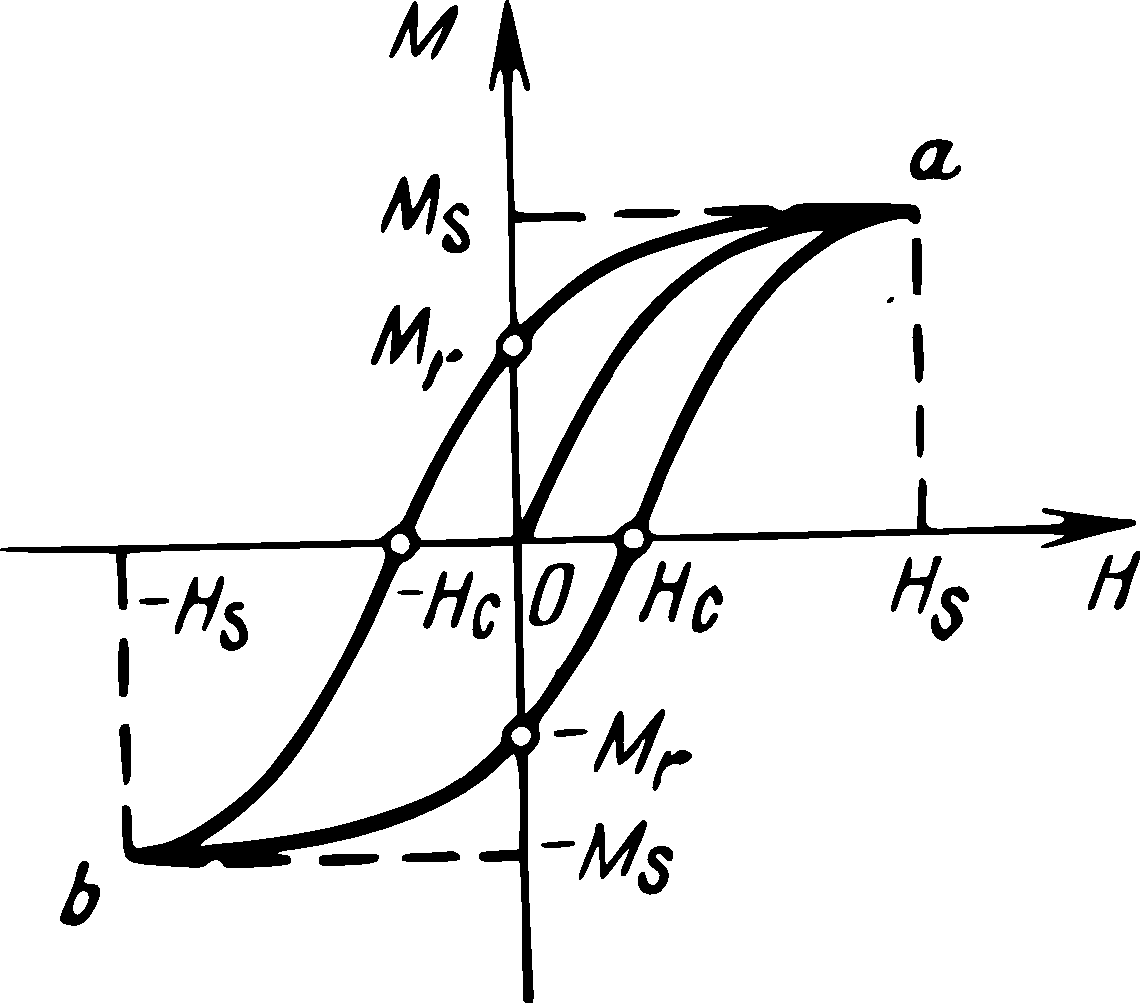
\includegraphics[width=0.8\textwidth]{figs/ch-26/fig-26-07.pdf}
\sidecaption{The hysteresis loop of a ferromagnetic material.\zhcap{铁磁性物质的磁滞回线。}\label{fig-26-07}}
\end{marginfigure}


The strength $\pm H_{c}$ of the external field that completely demagnetizes a substance is called the \redem{coercive force}. The coercive force specifies the property of a ferromagnetic material to retain its residual magnetization. \redem{Hard}, or \redem{retentive, magnetic materials} have a high coercive force. They have a wide hysteresis loop and are used to make permanent magnets. \redem{Soft}, or \redem{non-retentive, magnetic materials} have a low coercive force. They have a narrow hysteresis loop and are used to make trans­ former cores.
\zhpar{能使物质完全退磁的外磁场强度 $\pm H_{c}$ 称为\redem{矫顽力}。矫顽力表征铁磁性物质保持剩磁的能力。\redem{硬磁}（或称\redem{保磁性}）材料的矫顽力高，磁滞回线宽，用于制造永磁体。\redem{软磁}（或称\redem{非保磁性}）材料的矫顽力低，磁滞回线窄，用于制作变压器铁芯。}

The reversal of magnetization is associated with a change in the orientation of the regions of spontaneous magnetization \ssect{26.5.4} and requires that work be done at the expense of the energy of the external magnetic field. The amount of heat evolved in reversing magnetization is proportional to the area of the hysteresis loop.
\zhpar{磁化方向的反转与自发磁化区取向的改变有关，并需要以外磁场的能量为代价做功 \ssect{26.5.4}。反转磁化时放出的热量与磁滞回线的面积成正比。}

\subsection{}\label{26.5.4} At temperatures below the Curie point \ssect{26.5.2} a ferromagnetic material is made up of \redem{domains}, which are small \redem{regions of uniform spontaneous magnetization}. The linear dimensions of these domains range from \num{d-5} to \SI{d-4}{\meter}. Within each domain the substance is magnetized to saturation \ssect{26.5.2}. In the absence of an external magnetic field, the magnetic moments of the various domains are oriented in space so that the resultant magnetic moment of the whole ferromagnetic body equals zero.
\zhpar{在低于居里点的温度下（\ssect{26.5.2}），铁磁性物质由\redem{磁畴}组成。磁畴是微小的\redem{均匀自发磁化区}，其线度为 \num{d-5} 至 \SI{d-4}{\meter}。在每个磁畴内，物质都被磁化至饱和 \ssect{26.5.2}。在没有外磁场时，各磁畴的磁矩在空间中取向各异，使整个铁磁性物体的合磁矩为零。}

Owing to the effect of the external magnetic field, the magnetic moments of whole domains are oriented in a ferromagnetic material, rather than those of the separate particles as in the case of paramagnetic materials \ssect{26.3.6}. As a result, the sub­ stance is magnetized.
\zhpar{在外磁场的作用下，铁磁性物质中取向的是整个磁畴的磁矩，而不是像顺磁性物质那样取向单个粒子的磁矩 \ssect{26.3.6}。结果，物质被磁化。}

Ferromagnetic properties can only exist in the crystalline state of substances in which the interaction between the neighbouring atoms of the crystal lattice leads to the total energy of the system of electrons that provides for compliance with the conditions for the existence of ferromagnetism \ssect{26.5.1}.
\zhpar{铁磁性只能存在于晶态物质中：晶格中相邻原子之间的相互作用，使电子系统的总能量满足铁磁性存在的条件 \ssect{26.5.1}。}

\subsection{}\label{26.5.5} Measurement of the gyromagnetic ratio \ssect{26.1.4} for ferromagnetic bodies indicates that the elementary carriers of magnetism in ferromagnetic materials are the spin magnetic moments of the electrons \ssect{26.1.4}. The modern quantum mechanical theory of ferromagnetism explains the nature of the spontaneous magnetization of ferromagnetic materials \ssect{26.5.4} and the reasons for the development of a strong intrinsic magnetic field \ssect{26.4.1}.
\zhpar{对铁磁性物体旋磁比（\ssect{26.1.4}）的测量表明，铁磁性材料中磁性的基本载体是电子的自旋磁矩 \ssect{26.1.4}。现代铁磁性的量子力学理论阐明了铁磁性材料自发磁化的本质 \ssect{26.5.4}，以及产生强内禀磁场的原因 \ssect{26.4.1}。}

Ferromagnetic properties are possessed by crystals of substances whose atoms have inner shells and subshells \ssect{39.3.6} unfilled by electrons and having a nonzero value of the projections of the resultant spin moment on the direction of the magnetic field \ssect{26.1.3}. Developed between the spins of such electrons is a specific kind of quantum mechanical interaction that is not of a magnetic origin. It is called exchange interaction \ssect{39.4.5}. As a result, the state of the system of electrons in fer­ romagnetic materials is found to be stable upon parallel align­ ment of the spins, and spontaneous magnetization \ssect{26.5.4} is developed along with a strong intrinsic magnetic field.
\zhpar{铁磁性为具有下列特征的物质晶体所具有：其原子的内壳层和次壳层未被电子填满（\ssect{39.3.6}），且合自旋磁矩在磁场方向上的投影不为零（\ssect{26.1.3}）。这些电子的自旋之间形成一种特殊的量子力学相互作用，它并非磁性起源。该相互作用称为交换相互作用（\ssect{39.4.5}）。因此，铁磁性物质中电子系统的状态在自旋平行排列时最为稳定，并随之产生自发磁化 \ssect{26.5.4} 和强内禀磁场。}
